\RequirePackage[l2tabu,orthodox]{nag}

% TODO: decide if one-sided/two-sided
%\documentclass[headsepline,footsepline,footinclude=false,fontsize=11pt,paper=a4,listof=totoc,bibliography=totoc,BCOR=12mm,DIV=12]{scrbook} % two-sided
\documentclass[headsepline,footsepline,footinclude=false,oneside,fontsize=11pt,paper=a4,listof=totoc,bibliography=totoc]{scrbook} % one-sided

\PassOptionsToPackage{table,svgnames,dvipsnames}{xcolor}

\usepackage[utf8]{inputenc}
\usepackage[T1]{fontenc}
\usepackage[sc]{mathpazo}
\usepackage[american]{babel}
\usepackage[autostyle]{csquotes}
\usepackage[%
  backend=biber,
  url=false,
  style=alphabetic,
  maxnames=4,
  minnames=3,
  maxbibnames=99,
  firstinits,
  uniquename=init]{biblatex} % TODO: adapt bibliography style
\usepackage{graphicx}
\usepackage{scrhack} % necessary for listings package
\usepackage{listings}
\usepackage{lstautogobble}
\usepackage{tikz}
\usepackage{pgfplots}
\usepackage{pgfplotstable}
\usepackage{booktabs}
\usepackage[final]{microtype}
\usepackage{caption}
\usepackage[hidelinks]{hyperref} % hidelinks removes colored boxes around references and links
\usepackage[toc,nonumberlist,acronym]{glossaries} % TODO: remove if glossary not needed

\bibliography{bibliography/literature}

\setkomafont{disposition}{\normalfont\bfseries} % use serif font for headings
\linespread{1.05} % adjust line spread for mathpazo font

% Settings for glossaries TODO: remove the following block if glossary not needed
\renewcommand{\glsnamefont}[1]{\normalfont\bfseries #1} % use serif font for glossary entry titles
\makeglossaries{}

% Settings for pgfplots
\pgfplotsset{compat=1.9} % TODO: adjust to your installed version
\pgfplotsset{
  % For available color names, see http://www.latextemplates.com/svgnames-colors
  cycle list={CornflowerBlue\\Dandelion\\ForestGreen\\BrickRed\\},
}

% Settings for lstlistings
\lstset{%
  basicstyle=\ttfamily,
  columns=fullflexible,
  autogobble,
  keywordstyle=\bfseries\color{MediumBlue},
  stringstyle=\color{DarkGreen}
}

% Basic information for cover & title page
\newcommand*{\getUniversity}{Technische Universität München}
\newcommand*{\getFaculty}{Department of Informatics}
\newcommand*{\getTitle}{TODO: Thesis title}
\newcommand*{\getTitleGer}{TODO: Titel der Abschlussarbeit}
\newcommand*{\getAuthor}{TODO: Author}
\newcommand*{\getDoctype}{TODO: Thesis type (Bachelor's Thesis in Informatics, Master's Thesis in Robotics, \ldots)}
\newcommand*{\getSupervisor}{TODO: Supervisor}
\newcommand*{\getAdvisor}{TODO: Advisor}
\newcommand*{\getSubmissionDate}{TODO: Submission date}
\newcommand*{\getSubmissionLocation}{Munich}

% TODO: add custom commands etc.


% TODO: remove if glossary not needed
\newglossaryentry{computer}
{
  name=computer,
  description={is a machine that\ldots}
}

\newacronym{tum}{TUM}{Technische Universität München}


\newcolumntype{R}[1]{>{\raggedleft\let\newline\\\arraybackslash\hspace{0pt}}m{#1}}

\begin{document}

\begin{titlepage}
  % HACK for two-sided documents: ignore binding correction for cover page.
  % Adapted from Markus Kohm's KOMA-Script titlepage=firstiscover handling.
  % See http://mirrors.ctan.org/macros/latex/contrib/koma-script/scrkernel-title.dtx,
  % \maketitle macro.
  \oddsidemargin=\evensidemargin\relax
  \textwidth=\dimexpr\paperwidth-2\evensidemargin-2in\relax
  \hsize=\textwidth\relax

  \centering

  
\includegraphics[width=40mm]{logos/tum}

  \vspace{5mm}
  {\huge\MakeUppercase{\getFaculty{}}}\\

  \vspace{5mm}
  {\large\MakeUppercase{\getUniversity{}}}\\

  \vspace{20mm}
  {\Large Secure Coding Phase 2}
  %{\Large \getDoctype{}}

  \vspace{15mm}
  %{\huge\bfseries \getTitle{}}

  \vspace{15mm}
  {\LARGE Team 3:
  	 Patrick Sattler, Aurel Roci, Stefan Kohler}
  %{\LARGE \getAuthor{}}

  \vspace{20mm}
  
\includegraphics[width=20mm]{logos/faculty}
\end{titlepage}


\frontmatter{}


{
	\chapter{Executive Summary}\

   \textbf{Team2}\\

	We found several vulnerabilities, which could cause severe damage to the \textit{Team2}. It is possible to get access to the admin page via stealing the session. Thus an attacker can register an arbitrary employee or customer and unlock the registered user. There is also no upload format of the content, for the file to be uploaded.\\


	\textbf{Team3}\\

	We found some issues, which potentially could cause damage to the \textit{Team3 Online Banking}. However the detected issues are quite easy to fix. If an experienced attacker performs a man in the middle attack he'll be able to track session ids. The implications are severe, as the	attacker can take over the role of the customer, but this attack requires advanced knowledge. With regard to the business logic there was only one issue with low risk detected. \\

	\textbf{Comparison}\\

	In summary we were able to clearly state out that the \textit{Team3 Online Banking} web application has less and also less severe vulnerabilites then the \textit{Team2} web application. Furthermore it has to be said that the detected issues of the \textit{Team3 Online Banking} are easier to fix and will cost less money to implement.
}

\pagebreak
%\begin{titlepage}
  \centering

  
\includegraphics[width=40mm]{logos/tum}

  \vspace{5mm}
  {\huge\MakeUppercase{\getFaculty{}}}\\

  \vspace{5mm}
  {\large\MakeUppercase{\getUniversity{}}}\\
 
  \vspace{20mm}
  {\Large \getDoctype{}}

  \vspace{15mm}
  {\huge\bfseries \getTitle{}}

%  \vspace{10mm}
%  {\huge\bfseries \getTitleGer{}}

  \vspace{15mm}
%  \begin{tabular}{l l}
%    Author: & \getAuthor{} \\
%    Supervisor: & \getSupervisor{} \\
%    Advisor: & \getAdvisor{} \\
%    Submission Date: & \getSubmissionDate{} \\
%  \end{tabular}

  \vspace{20mm}
  
\includegraphics[width=20mm]{logos/faculty}
\end{titlepage}

%\thispagestyle{empty}
\vspace*{0.8\textheight}
\noindent
I confirm that this \MakeLowercase{\getDoctype{}} is my own work and I have documented all sources and material used.

\vspace{15mm}
\noindent
\getSubmissionLocation{}, \getSubmissionDate{} \hspace{5cm} \getAuthor{}

\cleardoublepage{}

%\addcontentsline{toc}{chapter}{Acknowledgments}
\thispagestyle{empty}

\vspace*{2cm}

\begin{center}
{\usekomafont{section} Acknowledgments}
\end{center}

\vspace{1cm}

%TODO: Acknowledgments

\cleardoublepage{}

%\chapter{\abstractname}

%TODO: Abstract



\microtypesetup{protrusion=false}
\tableofcontents{}
\microtypesetup{protrusion=true}
\mainmatter{}

\chapter{Time Tracking Table}

\begin{table}[htb]

	\centering
	\resizebox{9cm}{!}{%
	\begin{tabular}{lll}
		\hline
		{\textbf{Name}} & { \textbf{Task}} & {\textbf{Time}} \\ \hline
		Aurel Roci &  Configuration and Deploy Management Testing  &  1.5          \\
		
	    & Error Handling   &  0.25             \\
		& Testing for default credentials & 0.25  \\
		& Testing for Reflected Cross Site Scripting &  0.25  \\
		& Testing for Stored Cross Site Scripting   & 0.25 \\
		& Testing for HTTP Verb Tampering &  0.25     \\
		& Testing for SQL Injection &  0.25 \\
		& Test Number of Times a Function Can be Used Limits & 0.25 \\
		& Test Business Logic Data Validation & 1 \\
		& Executive Summary & 0.5 \\
		& Testing Report & 2  \\
		& Testing for Cross Site Request Forgery  & 0.25  \\
		& Testing for Privilege Escalation  & 1  \\
		& Presentation & 0.25 \\
		\hline
		\hline
		Stefan Ch. Kofler & \\
	
		\hline
		\hline
		Patrick Sattler &  \\
		& Presentation & 2 \\ 
		& Testing for Code Injection, local or remote file inclusion & 1 \\
		& Testing for Command Injection & 0.5 \\
		& Testing for Format string & 0.25 \\
		& Testing for incubated vulnerabilities & 0.5 \\
		 &  &
	\end{tabular}%
}
\end{table}

%\chapter{Introduction}\label{chapter:introduction}

\section{Section}
Citation test~\parencite{latex}.

\subsection{Subsection}
See~\autoref{fig:sample}.

\begin{figure}[htpb]
  \centering
  
\includegraphics{logos/tum}
  \caption[Example figure]{An example for a figure.}\label{fig:sample}
\end{figure}

\section{Section}

See~\autoref{tab:sample}, \autoref{fig:sample-drawing}, \autoref{fig:sample-plot}, \autoref{fig:sample-listing}.

\begin{table}[htpb]
  \caption[Example table]{An example for a simple table.}\label{tab:sample}
  \centering
  \begin{tabular}{l l l l}
    \toprule
      A & B & C & D \\
    \midrule
      1 & 2 & 1 & 2 \\
      2 & 3 & 2 & 3 \\
    \bottomrule
  \end{tabular}
\end{table}

\begin{figure}[htpb]
  \centering
  % This should probably go into a file in figures/
  \begin{tikzpicture}[node distance=3cm]
    \node (R0) {$R_1$};
    \node (R1) [right of=R0] {$R_2$};
    \node (R2) [below of=R1] {$R_4$};
    \node (R3) [below of=R0] {$R_3$};
    \node (R4) [right of=R1] {$R_5$};

    \path[every node]
      (R0) edge (R1)
      (R0) edge (R3)
      (R3) edge (R2)
      (R2) edge (R1)
      (R1) edge (R4);
  \end{tikzpicture}
  \caption[Example drawing]{An example for a simple drawing.}\label{fig:sample-drawing}
\end{figure}

\begin{figure}[htpb]
  \centering

  \pgfplotstableset{col sep=&, row sep=\\}
  % This should probably go into a file in data/
  \pgfplotstableread{
    a & b    \\
    1 & 1000 \\
    2 & 1500 \\
    3 & 1600 \\
  }\exampleA
  \pgfplotstableread{
    a & b    \\
    1 & 1200 \\
    2 & 800 \\
    3 & 1400 \\
  }\exampleB
  % This should probably go into a file in figures/
  \begin{tikzpicture}
    \begin{axis}[
        ymin=0,
        legend style={legend pos=south east},
        grid,
        thick,
        ylabel=Y,
        xlabel=X
      ]
      \addplot table[x=a, y=b]{\exampleA};
      \addlegendentry{Example A};
      \addplot table[x=a, y=b]{\exampleB};
      \addlegendentry{Example B};
    \end{axis}
  \end{tikzpicture}
  \caption[Example plot]{An example for a simple plot.}\label{fig:sample-plot}
\end{figure}

\begin{figure}[htpb]
  \centering
  \begin{tabular}{c}
  \begin{lstlisting}[language=SQL]
    SELECT * FROM tbl WHERE tbl.str = "str"
  \end{lstlisting}
  \end{tabular}
  \caption[Example listing]{An example for a source code listing.}\label{fig:sample-listing}
\end{figure}

% TODO: add more chapters here

\chapter{Vulnerabilities Overview}
Based on our testing, we identified the following vulnerabilities for the Team2
Bank and the OnlineBanking Bank:
\section{Team2}

\subsection{Static Session ID} \
\begin{itemize}
	\item Likelihood: \textit{high}
	\item Implication: \textit{high}
	\item Risk: \textit{high} 
\end{itemize}

The session id is saved in form of the (static) user id in a cookie. This cookie can be used on any machine
to take over the account of a user. The lifetime of this cookie is only limited by the cookie lifetime field.

\subsection{File Upload} 
There was no instructions on the structure of the information for the file upload functionality. There was a sample file, but after uploading it, and trying it with several accounts, it did not work.

\subsection{Mail}
The e-mail functionality to send the tans upon sign up was not working.


\section{Team3}

After testing the application there were no vulnerabilities found!

 

\chapter{Tools used}
\

\textit{sqlmap} - We used \textit{sqlmap} to test for SQL Injections, and we did not find any.\

\textit{RIPS} - We used RIPS to do a static testing of the PHP code. It showed warnings for SQL Injections which were \textit{false-positives}. The were also some \textit{false-positive} with command execution.\

\textit{FindBugs} - We used this tool to do a static testing of the Java code, and we did not find any vulnerabilities in the code of \textit{Team2}, and we found two \textit{false-positive} warnings in the code of \textit{Team3}.\

\textit{netcat} - We used this tool to check the HTTP methods but it did not give any output. \

\textit{nmap} We used this tool to check HTTP method, and it showed which methods were allowed and which ones were not allowed.

\textit{w3af} - We used this tool to find if the website had vulnerabilities by running an automatic test one the website. And found CSRF vulnerability. \

\textit{Zed Attack Proxy (ZAP)} - We used this for a spider attack towards the website, and did not find any CSRF vulnerability.\

\textit{Burp} - We used this tool to to intercept the message from the web browser to the server and alter it.\

\chapter{Detailed Report}

The following pages describe for each test how both applications Team2 and Team3. The test is divided in different sections following the OWASP Testing Guide v4.

\pagebreak


\section{Configuration and Deploy Management Testing}\
\subsection{Test File Extensions Handling for Sensitive Information (OTG-CONFIG-003)}\

\begin{tabular}{cR{12cm}}
	\textbf{Team2} & Likelihood: 8\\& Impact: 9\\& Risk: 3
\end{tabular}

\begin{tabular}{ l|p{11cm}  }
	\hline
	\multicolumn{2}{c}{\textbf{Team2}} \\
	\hline
	Observation   & File extensions are handled correctly but while testing we found folders which we could access.   \\
	Discovery  & TODO \\
	Likelihood & The likelihood is quite high that someone tries a tool to find these kind of vulnerabilities. There is no need for special knowledge because the tools work quite automatically without much configuration. \\
	Impact    & There is no impact the folders do not contain sensitive information.\\
	Recommendations & Block the access to files and to those folders, or remove them from the directory since they are not needed there.\\ 
	\hline
\end{tabular}
\\
\vspace{0.5cm}
\\
\begin{center}
	\begin{tabular}{ll}
		\rowcolor[HTML]{34CDF9}
		{\color[HTML]{ECF4FF} \textbf{Metric}}        & {\color[HTML]{ECF4FF} \textbf{Value : 9.8}} \\
		\rowcolor[HTML]{BBDAFF}
		{\color[HTML]{333333} Access Vector}          & {\color[HTML]{333333} } N              \\
		\rowcolor[HTML]{ECF4FF}
		{\color[HTML]{333333} Attack Complexity}      & {\color[HTML]{333333} } L              \\
		\rowcolor[HTML]{BBDAFF}
		{\color[HTML]{333333} Privileges Required}    & {\color[HTML]{333333} } N              \\
		\rowcolor[HTML]{ECF4FF}
		{\color[HTML]{333333} User Interaction}       & {\color[HTML]{333333} } N              \\
		\rowcolor[HTML]{BBDAFF}
		{\color[HTML]{333333} Scope}                  & {\color[HTML]{333333} } U              \\
		\rowcolor[HTML]{ECF4FF}
		{\color[HTML]{333333} Confidentiality Impact} & {\color[HTML]{333333} } H              \\
		\rowcolor[HTML]{BBDAFF}
		{\color[HTML]{333333} Integrity Impact}       & {\color[HTML]{333333} } H              \\
		\rowcolor[HTML]{ECF4FF}
		{\color[HTML]{333333} Availability Impact}    & {\color[HTML]{333333} } H
	\end{tabular}
\end{center}
\begin{tabular}{cR{12cm}}
	\textbf{Team3} & Likelihood: 8\\& Impact: 0\\& Risk: 1
\end{tabular}

\begin{tabular}{ l|p{11cm}  }
	\hline
	\multicolumn{2}{c}{\textbf{Team3}} \\
	\hline
	Observation   & File extensions are handled correctly but while testing we found folders which we could access smart-card simulator folder.   \\
	Discovery  & TODO \\
	Likelihood & The likelihood is quite high that someone tries a tool to find these kind of vulnerabilities. There is no need for special knowledge because the tools work quite automatically without much configuration. \\
	Impact    & There is no impact since there is nothing important hard-coded in the jave file.\\
	Recommendations & Block the access to files and to those folders.\\ 
	\hline
\end{tabular}

\begin{center}
	\begin{tabular}{ll}
		\rowcolor[HTML]{34CDF9}
		{\color[HTML]{ECF4FF} \textbf{Metric}}        & {\color[HTML]{ECF4FF} \textbf{Value : 0}} \\
		\rowcolor[HTML]{BBDAFF}
		{\color[HTML]{333333} Access Vector}          & {\color[HTML]{333333} } N              \\
		\rowcolor[HTML]{ECF4FF}
		{\color[HTML]{333333} Attack Complexity}      & {\color[HTML]{333333} } L              \\
		\rowcolor[HTML]{BBDAFF}
		{\color[HTML]{333333} Privileges Required}    & {\color[HTML]{333333} } N              \\
		\rowcolor[HTML]{ECF4FF}
		{\color[HTML]{333333} User Interaction}       & {\color[HTML]{333333} } N              \\
		\rowcolor[HTML]{BBDAFF}
		{\color[HTML]{333333} Scope}                  & {\color[HTML]{333333} } U              \\
		\rowcolor[HTML]{ECF4FF}
		{\color[HTML]{333333} Confidentiality Impact} & {\color[HTML]{333333} } N              \\
		\rowcolor[HTML]{BBDAFF}
		{\color[HTML]{333333} Integrity Impact}       & {\color[HTML]{333333} } N              \\
		\rowcolor[HTML]{ECF4FF}
		{\color[HTML]{333333} Availability Impact}    & {\color[HTML]{333333} } N
	\end{tabular}
\end{center}
\pagebreak

\subsection{Test HTTP Methods (OTG-CONFIG-006)}\


\begin{tabular}{cR{12cm}}
	\textbf{Team2} & Likelihood: 0\\& Impact: 0\\& Risk: 0
\end{tabular}

\begin{tabular}{ l|p{11cm}  }
	\hline
	\multicolumn{2}{c}{\textbf{Team2}} \\
	\hline
	Observation   &  The application is not accessable over HTTP. HTTPS is enforced.  \\
	Discovery  &  We also tried to connect via \textit{netcat} using the following command: \textit{{nc IP\_ADDRESS 80}} , which did not work. We also used \textit{nmap} for testing which returned the methods used by the webapp.\\

	Likelihood & N/A \\
	Implication    & N/A \\
	Recommendations & N/A \\
	Comparison &  The same applies for our web application.\\
	\hline
\end{tabular}

\begin{figure}[H]
	\centering
	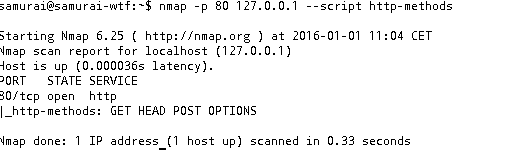
\includegraphics[width=150mm]{logos/nmap.jpg}
	\caption{RIPS \label{overflow}}
\end{figure} 

\pagebreak
\subsection{Test HTTP Strict Transport Security (OTG-CONFIG-007)}\
\begin{tabular}{cR{12cm}}
	\textbf{Team2} & Likelihood: 0\\& Impact: 0\\& Risk: 0
\end{tabular}

\begin{tabular}{ l|p{11cm}  }
	\hline
	\multicolumn{2}{c}{\textbf{Team2}} \\
	\hline
	Observation   &  The webapp is not using Strict Transport Security.  \\
	Discovery  &  We found this using \textit{Curl}.\\
	
	Likelihood & It is not complicated to perform a MitM attack to exploit this vulnerability. \\
	Impact    & A man-in-the-middle attacker attempts to intercept traffic from a victim user using an invalid certificate and hopes the user will accept the bad certificate. \\
	Recommendations & Enable Strict Transport Security. \\
	Comparison & Our webapp has Strict Transport Security enabled. \\
	\hline
\end{tabular}
 \begin{figure}[H]
 	\centering
 	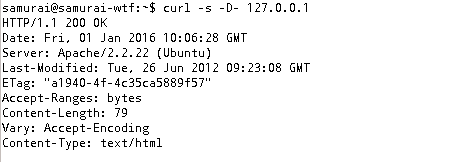
\includegraphics[width=150mm]{logos/rsts.jpg}
 	\caption{RIPS \label{overflow}}
 \end{figure} 
\pagebreak
\subsection{Test RIA cross domain policy (OTG-CONFIG-008)}\
\begin{tabular}{cR{12cm}}
	\textbf{Team2} & Likelihood: 0\\& Impact: 0\\& Risk: 0
\end{tabular}

\begin{tabular}{ l|p{11cm}  }
	\hline
	\multicolumn{2}{c}{\textbf{Team2}} \\
	\hline
	Observation   & There are no RIA applications on the system and therefore is no crossdomain.xml file provided. \\
	Discovery  & Using \textit{wget} we tried to find a \textit{crossdomain.xml} or \textit{clientaccesspolicy.xml} file and couldn't find it. \\
	Likelihood & N/A \\
	Implication    & N/A \\
	Recommendations & N/A \\
	Comparison & The same results applies for our web application. \\
	\hline
\end{tabular}
\\
\vspace{0.5cm}
\\
\begin{center}
	\begin{tabular}{ll}
		\rowcolor[HTML]{34CDF9}
		{\color[HTML]{ECF4FF} \textbf{Metric}}        & {\color[HTML]{ECF4FF} \textbf{Value}} \\
		\rowcolor[HTML]{BBDAFF}
		{\color[HTML]{333333} Access Vector}          & {\color[HTML]{333333} } N/A              \\
		\rowcolor[HTML]{ECF4FF}
		{\color[HTML]{333333} Attack Complexity}      & {\color[HTML]{333333} } N/A              \\
		\rowcolor[HTML]{BBDAFF}
		{\color[HTML]{333333} Privileges Required}    & {\color[HTML]{333333} } N/A              \\
		\rowcolor[HTML]{ECF4FF}
		{\color[HTML]{333333} User Interaction}       & {\color[HTML]{333333} } N/A              \\
		\rowcolor[HTML]{BBDAFF}
		{\color[HTML]{333333} Scope}                  & {\color[HTML]{333333} } N/A              \\
		\rowcolor[HTML]{ECF4FF}
		{\color[HTML]{333333} Confidentiality Impact} & {\color[HTML]{333333} } N/A              \\
		\rowcolor[HTML]{BBDAFF}
		{\color[HTML]{333333} Integrity Impact}       & {\color[HTML]{333333} } N/A              \\
		\rowcolor[HTML]{ECF4FF}
		{\color[HTML]{333333} Availability Impact}    & {\color[HTML]{333333} } N/A
	\end{tabular}
\end{center}
\pagebreak


\pagebreak
\section{Identity Management Testing}\
\subsection{Test Role Definitions (OTG-IDENT-001)}\
\begin{tabular}{cR{12cm}}
	\textbf{Team2} & Likelihood: 10\\& Impact: 0\\& Risk: 0
\end{tabular}

\begin{tabular}{ l|p{11cm}  }
	\hline
	\multicolumn{2}{c}{\textbf{Team2}} \\
	\hline
	Observation   & We found out that there exist two different roles in the system. There is the role of a normal customer and the role of an banker. Employees can view account and transaction details of all the customers. Transactions over 10000 euro and new user registrations can be accepted by the employee.\\
	Discovery  & All the roles and their available functions can be seen on the webapp.  \\
	Likelihood & It is very likely that people find this information. \\
	Impact    & There is no direct implication. \\
	Recommendations & N/A \\ 
	\hline
\end{tabular}
\\
\vspace{0.5cm}
\\
\begin{tabular}{cR{12cm}}
	\textbf{Team3} & Likelihood: 0\\& Impact: 0\\& Risk: 0
\end{tabular}

\begin{tabular}{ l|p{11cm}  }
	\hline
	\multicolumn{2}{c}{\textbf{Team3}} \\
	\hline
	Observation   & We found out that there exist two different roles in the system. There is the role of a normal customer and the role of an banker. Employees can view account and transaction details of all the customers. Transactions over 10000 euro and new user registrations can be accepted by the employee.\\
	Discovery  & All the roles and their available functions can be seen on the webapp.  \\
	Likelihood & It is very likely that people find this information. \\
	Impact    & There is no direct implication. \\
	Recommendations & N/A \\
	\hline
\end{tabular}
 
\pagebreak

\subsection{Test User Registration Process (OTG-IDENT-002)}\
\begin{tabular}{cR{12cm}}
	\textbf{Team2} & Likelihood: 5\\& Impact: 5\\& Risk: 5
\end{tabular}

\begin{tabular}{ l|p{11cm}  }
	\hline
	\multicolumn{2}{c}{\textbf{Team2}} \\
	\hline
	Observation   & Any person can register themselves as an user and this registration than gets validated by an employee. One person can register multiple times and with different roles. There is no proof of the identity of a user possible. The identification requirements include the email address and username, but only two of these can be verified. \\
	Discovery  & No special tools are needed to get this information. A browser and multiple registration tests provided the necessary results. \\
	Likelihood & It is quite likely that this information can be retrieved by any user with minimal experience. \\
	Implication    & User could try to register multiple times and with wrong information to get access to user accounts with more permissions or to create multiple bank accounts. \\
	Recommendations & The information passed in the registration form should be validated. The name can be validated by hand if a customer would go to the bank and the employee would than accept his registration. \\
	Comparison & Our web application doesn't require a phone number for the registration an the role of the user can be selected in the registration form. It doesn't make our application less secure, because the registration has still to be accepted by an employee. \\
	\hline
\end{tabular}
\\
\vspace{0.5cm}
\\
\begin{center}
	\begin{tabular}{ll}
		\rowcolor[HTML]{34CDF9}
		{\color[HTML]{ECF4FF} \textbf{Metric}}        & {\color[HTML]{ECF4FF} \textbf{Value}} \\
		\rowcolor[HTML]{BBDAFF}
		{\color[HTML]{333333} Access Vector}          & {\color[HTML]{333333} } N              \\
		\rowcolor[HTML]{ECF4FF}
		{\color[HTML]{333333} Attack Complexity}      & {\color[HTML]{333333} } L              \\
		\rowcolor[HTML]{BBDAFF}
		{\color[HTML]{333333} Privileges Required}    & {\color[HTML]{333333} } N              \\
		\rowcolor[HTML]{ECF4FF}
		{\color[HTML]{333333} User Interaction}       & {\color[HTML]{333333} } N              \\
		\rowcolor[HTML]{BBDAFF}
		{\color[HTML]{333333} Scope}                  & {\color[HTML]{333333} } U              \\
		\rowcolor[HTML]{ECF4FF}
		{\color[HTML]{333333} Confidentiality Impact} & {\color[HTML]{333333} } N              \\
		\rowcolor[HTML]{BBDAFF}
		{\color[HTML]{333333} Integrity Impact}       & {\color[HTML]{333333} } N              \\
		\rowcolor[HTML]{ECF4FF}
		{\color[HTML]{333333} Availability Impact}    & {\color[HTML]{333333} } N
	\end{tabular}
\end{center}
\pagebreak

\subsection{Test Account Provisioning Process (OTG-IDENT-003)}\
\begin{tabular}{cR{12cm}}
	\textbf{Team2} & Likelihood: N/A\\& Impact: N/A\\& Risk: N/A
\end{tabular}

\begin{tabular}{ l|p{11cm}  }
	\hline
	\multicolumn{2}{c}{\textbf{Team2}} \\
	\hline
	Observation   & Our observation showed us that employees can accept customer registrations. \\
	Discovery  & All the observations were made with the \textit{Chrome} web browser. \\
	Impact    & If an employee account gets hacked you can accept new registrations. \\
	Recommendations & N/A \\
	Comparison & In our web application the employee accepts new registration. It makes no difference in the security. \\
	\hline
\end{tabular}
\\
\vspace{0.5cm}
\\
\begin{center}
	\begin{tabular}{ll}
		\rowcolor[HTML]{34CDF9}
		{\color[HTML]{ECF4FF} \textbf{Metric}}        & {\color[HTML]{ECF4FF} \textbf{Value}} \\
		\rowcolor[HTML]{BBDAFF}
		{\color[HTML]{333333} Access Vector}          & {\color[HTML]{333333} } N/A              \\
		\rowcolor[HTML]{ECF4FF}
		{\color[HTML]{333333} Attack Complexity}      & {\color[HTML]{333333} } N/A              \\
		\rowcolor[HTML]{BBDAFF}
		{\color[HTML]{333333} Privileges Required}    & {\color[HTML]{333333} } N/A              \\
		\rowcolor[HTML]{ECF4FF}
		{\color[HTML]{333333} User Interaction}       & {\color[HTML]{333333} } N/A              \\
		\rowcolor[HTML]{BBDAFF}
		{\color[HTML]{333333} Scope}                  & {\color[HTML]{333333} } N/A              \\
		\rowcolor[HTML]{ECF4FF}
		{\color[HTML]{333333} Confidentiality Impact} & {\color[HTML]{333333} } N/A              \\
		\rowcolor[HTML]{BBDAFF}
		{\color[HTML]{333333} Integrity Impact}       & {\color[HTML]{333333} } N/A              \\
		\rowcolor[HTML]{ECF4FF}
		{\color[HTML]{333333} Availability Impact}    & {\color[HTML]{333333} } N/A
	\end{tabular}
\end{center}
\pagebreak

\subsection{Testing for Account Enumeration and Guessable User Account (OTG-IDENT-004)}\
\begin{tabular}{cR{12cm}}
	\textbf{Team2} & Likelihood: 0\\& Impact: 0\\& Risk: 0
\end{tabular}

\begin{tabular}{ l|p{11cm}  }
	\hline
	\multicolumn{2}{c}{\textbf{Team2}} \\
	\hline
	Observation   & We found out that the web application makes no difference between existing usernames and non existing usernames when trying to login with wrong credentials. The same html response and the same response headers are provided by the system. \\
	Discovery  & We used the \textit{Charles Web Proxy} to analyze the web application responses. \\
	Implication    & N/A \\
	Recommendations & N/A \\
	Comparison & Our web application makes no difference between login tries with existing usernames and non existing ones. Both web applications aren't vulnerable here. \\
	\hline
\end{tabular}
 
\pagebreak

\subsection{Testing for Weak or unenforced username policy (OTG-IDENT-005)}\
\begin{tabular}{cR{12cm}}
	\textbf{Team2} & Likelihood: 0\\& Impact: 0\\& Risk: 0
\end{tabular}

\begin{tabular}{ l|p{11cm}  }
	\hline
	\multicolumn{2}{c}{\textbf{Team2}} \\
	\hline
	Observation   & The usernames should be more than 2 characters. \\
	Discovery  & No tool is used here. Trying to sign up with short usernames gave us the warning. \\
	Impact   & N/A \\
	Recommendations & N/A \\
	Comparison & Our application has no username restriction. \\
	\hline
\end{tabular}
 
\pagebreak

\section{Authentication Testing}\
\subsection{Testing for Credentials Transported over an Encrypted Channel(OTG-AUTHN-001)}\

\begin{tabular}{cR{12cm}}
	\textbf{Team2} & Likelihood: 0\\& Impact: 0\\& Risk: 0
\end{tabular}

\begin{tabular}{ l|p{11cm}  }
	\hline
	\multicolumn{2}{c}{\textbf{Team2}} \\
	\hline
	Observation   & The webapp uses HTTPS protocol, so all the information is sent encrypted through the channel therefore we cannot sniff the data.\\
	Discovery  & The website s using an SSL certificate \\
	Likelihood & NA \\
	Impact    & NA\\
	Recommendations &   \\
	Comparison & Our webapp is using HTTPS, so the data is transported over an encrypted channel.\\
	\hline
\end{tabular}
\\
\vspace{0.5cm}
\\


\pagebreak
\subsection{Testing for default credentials(OTG-AUTHN-002)}\
\begin{tabular}{cR{12cm}}
	\textbf{Team2} & Likelihood: 10\\& Impact: 4\\& Risk: 6
\end{tabular}

\begin{tabular}{ l|p{11cm}  }
	\hline
	\multicolumn{2}{c}{\textbf{Team2}} \\
	\hline
	Observation   & There are no default credentials for the webapp. \\
	Discovery  & We saw the credentials text file that was given by the other team.\\
	Likelihood & N/A \\
	Impact    &  N/A \\
	Recommendations &  N/A\\
	Comparison & The same goes for our webapp.\\
	\hline
\end{tabular}
\pagebreak
\subsection{Testing for Weak lock out mechanism(OTG-AUTHN-003)}\
\begin{tabular}{cR{12cm}}
	\textbf{Team2} & Likelihood: 0\\& Impact: 0\\& Risk: 0
\end{tabular}

\begin{tabular}{ l|p{11cm}  }
	\hline
	\multicolumn{2}{c}{\textbf{Team2}} \\
	\hline
	Observation   & The user is shown redirected from the login page after a 3 failed tries. \\
	Discovery  &We entered the wrong credentials until we had to click the login button to be able to enter the credentials again.\\
	Likelihood & N/A \\
	Impact    &  N/A \\
	Recommendations &  N/A\\
	Comparison & The same goes for our webapp.\\
	\hline
\end{tabular}

\pagebreak
\subsection{Testing for bypassing authentication schema (OTG-AUTHN-004)}\

\begin{tabular}{cR{12cm}}
	\textbf{Team2} & Likelihood: NA\\& Impact: NA\\& Risk: NA
\end{tabular}

\begin{tabular}{ l|p{11cm}  }
	\hline
	\multicolumn{2}{c}{\textbf{Team2}} \\
	\hline
	Observation &  We did not find any possibility to bypass the authentication schema.\\
	Discovery & N/A\\
	Likelihood & N/A\\
	Implication & N/A\\
	Recommendations & N/A\\
	Comparison & Neither we found a possibility in our web app \\
	\hline
\end{tabular}
\\
\vspace{0.5cm}
\\
\begin{center}
	\begin{tabular}{ll}
		\rowcolor[HTML]{34CDF9}
		{\color[HTML]{ECF4FF} \textbf{Metric}}        & {\color[HTML]{ECF4FF} \textbf{Value}} \\
		\rowcolor[HTML]{BBDAFF}
		{\color[HTML]{333333} Access Vector}          & {\color[HTML]{333333} } NA              \\
		\rowcolor[HTML]{ECF4FF}
		{\color[HTML]{333333} Attack Complexity}      & {\color[HTML]{333333} } NA              \\
		\rowcolor[HTML]{BBDAFF}
		{\color[HTML]{333333} Privileges Required}    & {\color[HTML]{333333} } NA              \\
		\rowcolor[HTML]{ECF4FF}
		{\color[HTML]{333333} User Interaction}       & {\color[HTML]{333333} } NA              \\
		\rowcolor[HTML]{BBDAFF}
		{\color[HTML]{333333} Scope}                  & {\color[HTML]{333333} } NA              \\
		\rowcolor[HTML]{ECF4FF}
		{\color[HTML]{333333} Confidentiality Impact} & {\color[HTML]{333333} } NA              \\
		\rowcolor[HTML]{BBDAFF}
		{\color[HTML]{333333} Integrity Impact}       & {\color[HTML]{333333} } NA              \\
		\rowcolor[HTML]{ECF4FF}
		{\color[HTML]{333333} Availability Impact}    & {\color[HTML]{333333} } NA
	\end{tabular}
\end{center}

\pagebreak
\subsection{Testing for Browser cache weakness (OTG-AUTHN-006)}\

\begin{tabular}{cR{12cm}}
	\textbf{Team2} & Likelihood: 0\\& Impact: NA\\& Risk: NA
\end{tabular}

\begin{tabular}{ l|p{11cm}  }
	\hline
	\multicolumn{2}{c}{\textbf{Team2}} \\
	\hline
	Observation & The web app set the cache-control to no-cache an no-store and Pragma to no-cache\\
	Discovery & By checking the \textit{about:cache} in Firefox we saw the Headers\\
	Likelihood &  N/A \\
	Implication & N/A \\
	Recommendations &  N/A\\
	Comparison & The same goes for our webapp \\
	\hline
\end{tabular}
\\
\vspace{0.5cm}
\\
\begin{center}
	\begin{tabular}{ll}
		\rowcolor[HTML]{34CDF9}
		{\color[HTML]{ECF4FF} \textbf{Metric}}        & {\color[HTML]{ECF4FF} \textbf{Value}} \\
		\rowcolor[HTML]{BBDAFF}
		{\color[HTML]{333333} Access Vector}          & {\color[HTML]{333333} } NA              \\
		\rowcolor[HTML]{ECF4FF}
		{\color[HTML]{333333} Attack Complexity}      & {\color[HTML]{333333} } NA              \\
		\rowcolor[HTML]{BBDAFF}
		{\color[HTML]{333333} Privileges Required}    & {\color[HTML]{333333} } NA              \\
		\rowcolor[HTML]{ECF4FF}
		{\color[HTML]{333333} User Interaction}       & {\color[HTML]{333333} } NA              \\
		\rowcolor[HTML]{BBDAFF}
		{\color[HTML]{333333} Scope}                  & {\color[HTML]{333333} } NA              \\
		\rowcolor[HTML]{ECF4FF}
		{\color[HTML]{333333} Confidentiality Impact} & {\color[HTML]{333333} } NA              \\
		\rowcolor[HTML]{BBDAFF}
		{\color[HTML]{333333} Integrity Impact}       & {\color[HTML]{333333} } NA              \\
		\rowcolor[HTML]{ECF4FF}
		{\color[HTML]{333333} Availability Impact}    & {\color[HTML]{333333} } NA
	\end{tabular}
\end{center}

\pagebreak
\subsection{Testing for Weak password policy (OTG-AUTHN-007)}\

\begin{tabular}{cR{12cm}}
	\textbf{Team2} & Likelihood: 6\\& Impact: 5\\& Risk: 5
\end{tabular}

\begin{tabular}{ l|p{11cm}  }
	\hline
	\multicolumn{2}{c}{\textbf{Team2}} \\
	\hline
	Observation & The registration process does not have a restriction for weak passwords. Furthermore the password can contain the username\\
	Discovery & Tested manually the registration process with a one character password and the username as password\\
	Likelihood & For every registration process the user has the possibility to choose a weak password\\
	Implication & Brute Force is to easy for simple passwords\\
	Recommendations & Introduce password restrictions\\
	Comparison & The same problem we encountered in our webapp \\
	\hline
\end{tabular}
\\
\vspace{0.5cm}
\\
\begin{center}
	\begin{tabular}{ll}
		\rowcolor[HTML]{34CDF9}
		{\color[HTML]{ECF4FF} \textbf{Metric}}        & {\color[HTML]{ECF4FF} \textbf{Value}} \\
		\rowcolor[HTML]{BBDAFF}
		{\color[HTML]{333333} Access Vector}          & {\color[HTML]{333333} } N              \\
		\rowcolor[HTML]{ECF4FF}
		{\color[HTML]{333333} Attack Complexity}      & {\color[HTML]{333333} } L              \\
		\rowcolor[HTML]{BBDAFF}
		{\color[HTML]{333333} Privileges Required}    & {\color[HTML]{333333} } N              \\
		\rowcolor[HTML]{ECF4FF}
		{\color[HTML]{333333} User Interaction}       & {\color[HTML]{333333} } N              \\
		\rowcolor[HTML]{BBDAFF}
		{\color[HTML]{333333} Scope}                  & {\color[HTML]{333333} } U              \\
		\rowcolor[HTML]{ECF4FF}
		{\color[HTML]{333333} Confidentiality Impact} & {\color[HTML]{333333} } L              \\
		\rowcolor[HTML]{BBDAFF}
		{\color[HTML]{333333} Integrity Impact}       & {\color[HTML]{333333} } L              \\
		\rowcolor[HTML]{ECF4FF}
		{\color[HTML]{333333} Availability Impact}    & {\color[HTML]{333333} } N
	\end{tabular}
\end{center}

\pagebreak
\subsection{Testing for weak password change or reset functionalities (OTG-AUTHN-009)}\
\begin{tabular}{cR{12cm}}
	\textbf{Team2} & Likelihood: 10\\& Impact: 8\\& Risk: 5
\end{tabular}

\begin{tabular}{ l|p{11cm}  }
	\hline
	\multicolumn{2}{c}{\textbf{Team2}} \\
	\hline
	Observation & The password reset functionality can cause unwanted password change or the user to loose access to their account. Since the functionality changes the current password to a random one and sends an email to the user with the new password. \\
	Discovery & Tested manually to reset the password. An error occurred and the email was not send but the password was changed.\\
	Likelihood & It is very high that someone can enter an email address of another user and cause change their password without the users request.\\
	Impact & The impact can be quite high especially in case when the email with the new password fails to send, the user can loose access to his account.\\
	Recommendations & Instead of setting a new random password, sending an email with a link where the user can set a new password himself will be the best solution.\\
	Comparison & Our webapp  sends an email with link to change the password. The random number generated for the link is long, so trying to brute force it will take a very long time.\\ 
	\hline
\end{tabular}
\\
\vspace{0.5cm}
\\
\begin{center}
	\begin{tabular}{ll}
		\rowcolor[HTML]{34CDF9}
		{\color[HTML]{ECF4FF} \textbf{Metric}}        & {\color[HTML]{ECF4FF} \textbf{Value : 7.5 }} \\
		\rowcolor[HTML]{BBDAFF}
		{\color[HTML]{333333} Access Vector}          & {\color[HTML]{333333} } N              \\
		\rowcolor[HTML]{ECF4FF}
		{\color[HTML]{333333} Attack Complexity}      & {\color[HTML]{333333} } L              \\
		\rowcolor[HTML]{BBDAFF}
		{\color[HTML]{333333} Privileges Required}    & {\color[HTML]{333333} } N              \\
		\rowcolor[HTML]{ECF4FF}
		{\color[HTML]{333333} User Interaction}       & {\color[HTML]{333333} } N              \\
		\rowcolor[HTML]{BBDAFF}
		{\color[HTML]{333333} Scope}                  & {\color[HTML]{333333} } U              \\
		\rowcolor[HTML]{ECF4FF}
		{\color[HTML]{333333} Confidentiality Impact} & {\color[HTML]{333333} } N              \\
		\rowcolor[HTML]{BBDAFF}
		{\color[HTML]{333333} Integrity Impact}       & {\color[HTML]{333333} } N              \\
		\rowcolor[HTML]{ECF4FF}
		{\color[HTML]{333333} Availability Impact}    & {\color[HTML]{333333} } H
	\end{tabular}
\end{center}

\pagebreak
\section{Authorization Testing}\
\subsection{Testing Directory traversal/file include (OTG-AUTHZ-001)}\

\begin{tabular}{cR{12cm}}
	\textbf{Team2} & Likelihood: 0\\& Impact: 0\\& Risk: 0 
\end{tabular}

\begin{tabular}{ l|p{11cm}  }
	\hline
	\multicolumn{2}{c}{\textbf{Team2}} \\
	\hline
	Observation   & We could not find any path traversals .\\
	Discovery  & We used the \textit{dotdotpwn} tool to find such traversals with the following command:
	\begin{lstlisting}
		sudo ./dotdotpwn.pl -O -m http -h IP_ADDRESS 
	\end{lstlisting}
	-O is to get the operating system;  
	-m is to indicate that the protocol is http and -h for the server ip;  
	which gave no results.
	Afterwards we tried \textit{w3af} and it did not find anything.\\
	Likelihood & This is more an additional information for other attacks but it is a
	good help for attackers to find vulnerabilities faster \\
	Impact    & N/A \\
	Recommendations & N/A \\
	Comparison & The results were the same for our webapp.\\
	\hline
\end{tabular}  
 
\pagebreak

\subsection{Testing for Privilege Escalation (OTG-AUTHZ-003)}\

\begin{tabular}{cR{12cm}}
	\textbf{Team2} & Likelihood: 0\\& Impact: 0\\& Risk: 0
\end{tabular}

\begin{tabular}{ l|p{11cm}  }
	\hline
	\multicolumn{2}{c}{\textbf{Team2}} \\
	\hline
	Observation   & It is not possible to escalate privileges of the user.  \\
	Discovery  & We tried to change the user privilege by changing the user id after we saw that they are generated by incrementing from the first user ID, using \textit{Burp}.\\
	Likelihood & N/A \\
	Implication    & N/A \\
	Recommendations & N/A \\
	Comparison & The same results apply for our web application.\\
	\hline
\end{tabular}
\pagebreak

\subsection{Testing for Insecure Direct Object References (OTG-AUTHZ-004)}\
\begin{tabular}{cR{12cm}}
	\textbf{Team2} & Likelihood: 0\\& Impact: 0\\& Risk: 0
\end{tabular}

\begin{tabular}{ l|p{11cm}  }
	\hline
	\multicolumn{2}{c}{\textbf{Team2}} \\
	\hline
	Observation   & It is not possible to retrieve objects belonging to other users or otherwise bypass authorization.  \\
	Discovery  & We tried to change the user privilege by changing the user id after we saw that they are generated by incrementing from the first user ID, using \textit{Burp}.\\
	Likelihood & N/A \\
	Implication    & N/A \\
	Recommendations & N/A \\
	Comparison & The same results apply for our web application.\\
	\hline
\end{tabular}
\pagebreak
\section{Session Management Testing}\
\subsection{Testing for Bypassing Session Management Schema(OTG-SESS-001)}\

\begin{tabular}{cR{12cm}}
	\textbf{Team2} & Likelihood: 10\\ & Impact: 7\\& Risk: 7
\end{tabular}

\begin{tabular}{ l|p{11cm}  }
	\hline
	\multicolumn{2}{c}{\textbf{Team2}} \\
	\hline
	Observation   & There is no Random Session Token generated, nor any Session Time-out functionality. Also there is no cookie configuration.\\
	Discovery  & We observed the php code which we were given.\\
	Likelihood & It is very likely that an attacker notices this, since the SessionID does not change.\\
	Impact    & This can cause a Session Hijack.\\
	Recommendations & Generate random SessionIDs and create a Session Time-out functionality.\\
	Comparison& Our web app generates random SessionIDs creates a session time-out, also set the cookie parameters. \\
	\hline
\end{tabular}
\\
\vspace{0.5cm}
\\
\begin{center}
	\begin{tabular}{ll}
		\rowcolor[HTML]{34CDF9}
		{\color[HTML]{ECF4FF} \textbf{Metric}}        & {\color[HTML]{ECF4FF} \textbf{Value : 6.7}} \\
		\rowcolor[HTML]{BBDAFF}
		{\color[HTML]{333333} Access Vector}          & {\color[HTML]{333333} } L              \\
		\rowcolor[HTML]{ECF4FF}
		{\color[HTML]{333333} Attack Complexity}      & {\color[HTML]{333333} } H              \\
		\rowcolor[HTML]{BBDAFF}
		{\color[HTML]{333333} Privileges Required}    & {\color[HTML]{333333} } N              \\
		\rowcolor[HTML]{ECF4FF}
		{\color[HTML]{333333} User Interaction}       & {\color[HTML]{333333} } N              \\
		\rowcolor[HTML]{BBDAFF}
		{\color[HTML]{333333} Scope}                  & {\color[HTML]{333333} } U 	              \\
		\rowcolor[HTML]{ECF4FF}
		{\color[HTML]{333333} Confidentiality Impact} & {\color[HTML]{333333} } H              \\
		\rowcolor[HTML]{BBDAFF}
		{\color[HTML]{333333} Integrity Impact}       & {\color[HTML]{333333} } H              \\
		\rowcolor[HTML]{ECF4FF}
		{\color[HTML]{333333} Availability Impact}    & {\color[HTML]{333333} } N
	\end{tabular}
\end{center}

\pagebreak
\subsection{Testing for Cookies attributes(OTG-SESS-002)}\

\begin{tabular}{cR{12cm}}
	\textbf{Team2} & Likelihood: 10\\& Impact: 6\\& Risk: 3
\end{tabular}


\begin{tabular}{ l|p{11cm}  }
	\hline
	\multicolumn{2}{c}{\textbf{Team2}} \\
	\hline
	Observation &  The cookie for the PHP session id has a to general path (``//''). So
	the application is vulnerable to other web application on the same server. They will
	also get the cookie from the user.  The HttpOnly is not set also there is no expiration time for the cookie.\\
	Discovery  & We used the Firefox Web developer toolbar to analyze the cookie attributes. \\
	Likelihood & It is vary easy and straight forward to use this tool so it is highly likely for someone to find that out.\\
	Impact    & The cookies can be read and used by other web applications that
	match the path value. \\
	Recommendations & Set the path as tight as possible. \\
	Comparison & Our web app has the all the cookie parameters set, and the timeout of the cookie is set to 10 minutes.\\
	\hline
\end{tabular}
\\
\vspace{0.5cm}
\\
\begin{center}
	\begin{tabular}{ll}
		\rowcolor[HTML]{34CDF9}
		{\color[HTML]{ECF4FF} \textbf{Metric}}        & {\color[HTML]{ECF4FF} \textbf{Value : 6.1}} \\
		\rowcolor[HTML]{BBDAFF}
		{\color[HTML]{333333} Access Vector}          & {\color[HTML]{333333} } L             \\
		\rowcolor[HTML]{ECF4FF}
		{\color[HTML]{333333} Attack Complexity}      & {\color[HTML]{333333} } L              \\
		\rowcolor[HTML]{BBDAFF}
		{\color[HTML]{333333} Privileges Required}    & {\color[HTML]{333333} } N              \\
		\rowcolor[HTML]{ECF4FF}
		{\color[HTML]{333333} User Interaction}       & {\color[HTML]{333333} } R              \\
		\rowcolor[HTML]{BBDAFF}
		{\color[HTML]{333333} Scope}                  & {\color[HTML]{333333} } U              \\
		\rowcolor[HTML]{ECF4FF}
		{\color[HTML]{333333} Confidentiality Impact} & {\color[HTML]{333333} } H              \\
		\rowcolor[HTML]{BBDAFF}
		{\color[HTML]{333333} Integrity Impact}       & {\color[HTML]{333333} } L              \\
		\rowcolor[HTML]{ECF4FF}
		{\color[HTML]{333333} Availability Impact}    & {\color[HTML]{333333} } N
	\end{tabular}
\end{center}

\pagebreak
\subsection{Testing for Session Fixation(OTG-SESS-003)}\

\begin{tabular}{cR{12cm}}
	\textbf{Team2} & Likelihood: 9\\& Impact: 5\\& Risk: 5
\end{tabular}

\begin{tabular}{ l|p{11cm}  }
	\hline
	\multicolumn{2}{c}{\textbf{Team2}} \\
	\hline
	Observation   & The session id is not invalidated and therefore does not change after the user is authenticated. This means
	an attacker can force a known session id on a user. Once the user is authenticated the attacker can access also as authenticated
	user \\
	Discovery  & We used \textit{ZAP} proxy to intercept the traffic.\\
	Likelihood & This attack is pretty easy and can also be performed by low skilled people\\
	Implication    & The attacker can do everything the user can \\
	Recommendations& Change the session id after logging in \\
	Comparison & Our web app generates a new random SessionID after the user logs in.\\
	\hline
\end{tabular}
\\
\vspace{0.5cm}
\\
\begin{center}
	\begin{tabular}{ll}
		\rowcolor[HTML]{34CDF9}
		{\color[HTML]{ECF4FF} \textbf{Metric}}        & {\color[HTML]{ECF4FF} \textbf{Value : 8.1}} \\
		\rowcolor[HTML]{BBDAFF}
		{\color[HTML]{333333} Access Vector}          & {\color[HTML]{333333} } N             \\
		\rowcolor[HTML]{ECF4FF}
		{\color[HTML]{333333} Attack Complexity}      & {\color[HTML]{333333} } L              \\
		\rowcolor[HTML]{BBDAFF}
		{\color[HTML]{333333} Privileges Required}    & {\color[HTML]{333333} } N              \\
		\rowcolor[HTML]{ECF4FF}
		{\color[HTML]{333333} User Interaction}       & {\color[HTML]{333333} } R              \\
		\rowcolor[HTML]{BBDAFF}
		{\color[HTML]{333333} Scope}                  & {\color[HTML]{333333} } U              \\
		\rowcolor[HTML]{ECF4FF}
		{\color[HTML]{333333} Confidentiality Impact} & {\color[HTML]{333333} } H              \\
		\rowcolor[HTML]{BBDAFF}
		{\color[HTML]{333333} Integrity Impact}       & {\color[HTML]{333333} } H              \\
		\rowcolor[HTML]{ECF4FF}
		{\color[HTML]{333333} Availability Impact}    & {\color[HTML]{333333} } N
	\end{tabular}
\end{center}
\pagebreak
\subsection{Testing for Exposed Session Variables (OTG-SESS-004)}\

\begin{tabular}{cR{12cm}}
	\textbf{Team2} & Likelihood: 10\\& Impact: 6\\& Risk: 6
\end{tabular}

\begin{tabular}{ l|p{11cm}  }
	\hline
	\multicolumn{2}{c}{\textbf{Team2}} \\
	\hline
	Observation & The application from Team 2  use SSL certificate and therefore the session variables
	are not accessible during transport. But the Session variable is not destroyed after the user logs out.\\
	Discovery & We used the \textit{Firefox web developer tools} to analyze the cookies. Also the \textit{Firebug} tool and we got the same outcome. \\
	Likelihood & This attack is pretty easy and can also be performed by low skilled people\\
	Impact & The attacker can read the session variables and depending on the information in them  \\
	Recommendations & Remove the cookie after logout.\\
	Comparison & Our application destroys the session after the user logs out.\\
	\hline
\end{tabular}
\\
\vspace{0.5cm}
\\
\begin{center}
	\begin{tabular}{ll}
		\rowcolor[HTML]{34CDF9}
		{\color[HTML]{ECF4FF} \textbf{Metric}}        & {\color[HTML]{ECF4FF} \textbf{Value : 5.9}} \\
		\rowcolor[HTML]{BBDAFF}
		{\color[HTML]{333333} Access Vector}          & {\color[HTML]{333333} } P             \\
		\rowcolor[HTML]{ECF4FF}
		{\color[HTML]{333333} Attack Complexity}      & {\color[HTML]{333333} } L              \\
		\rowcolor[HTML]{BBDAFF}
		{\color[HTML]{333333} Privileges Required}    & {\color[HTML]{333333} } N              \\
		\rowcolor[HTML]{ECF4FF}
		{\color[HTML]{333333} User Interaction}       & {\color[HTML]{333333} } R              \\
		\rowcolor[HTML]{BBDAFF}
		{\color[HTML]{333333} Scope}                  & {\color[HTML]{333333} } U              \\
		\rowcolor[HTML]{ECF4FF}
		{\color[HTML]{333333} Confidentiality Impact} & {\color[HTML]{333333} } H              \\
		\rowcolor[HTML]{BBDAFF}
		{\color[HTML]{333333} Integrity Impact}       & {\color[HTML]{333333} } H              \\
		\rowcolor[HTML]{ECF4FF}
		{\color[HTML]{333333} Availability Impact}    & {\color[HTML]{333333} } N
	\end{tabular}
\end{center}
\pagebreak
\subsection{Testing for Cross Site Request Forgery(OTG-SESS-005)}\
\begin{tabular}{cR{12cm}}
	\textbf{Team2} & Likelihood: 10\\& Impact: 6\\& Risk: 6
\end{tabular}

\begin{tabular}{ l|p{11cm}  }
	\hline
	\multicolumn{2}{c}{\textbf{Team2}} \\
	\hline
	Observation & The application is vulnerable to CRSF.\\
	Discovery & WE used \textit{w3af} tool to analyze the website and it showed that there is CRSF vulnerability.\\
	Likelihood & N/A\\
	Impact & N/A  \\
	Recommendations & N/A\\
	Comparison & N/A\\
	\hline
\end{tabular}

\pagebreak
\subsection{Testing for logout functionality(OTG-SESS-006)}\

\begin{tabular}{cR{12cm}}
	\textbf{Team2} & Likelihood: 4\\& Impact: 6\\& Risk: 5
\end{tabular}

\begin{tabular}{ l|p{11cm}  }
	\hline
	\multicolumn{2}{c}{\textbf{Team2}} \\
	\hline
	Observation & The logout functionallity has been tested an works without any problems.
	The user gets correctly logged out and pages where authentication is needed can't be accessed afterwards.
	Also reusing the session id does not work. But the application seems to have no automatic
	logout after a certain amount of time.\\
	Discovery & We tested the functionallity manually and used the Chrome extension ``Advanced Rest Client'' to reuse the session cookie \\
	Likelihood & The only problem is that user sometimes only close the browser tab and than the session continues to exist.\\
	Impact & An attacker would be logged in if he can access afterwards the computer. Possible scenario Internet cafe	or something similar\\
	Recommendations & implement an automatic server side logout\\
	Comparison & Our webapp has the same problem that it does not log out after the web browser is closed, but it does log out after 10 minutes of inactivity.\\
	\hline
\end{tabular}
\\
\vspace{0.5cm}
\\
\begin{center}
	\begin{tabular}{ll}
		\rowcolor[HTML]{34CDF9}
		{\color[HTML]{ECF4FF} \textbf{Metric}}        & {\color[HTML]{ECF4FF} \textbf{Value : 4.6}} \\
		\rowcolor[HTML]{BBDAFF}
		{\color[HTML]{333333} Access Vector}          & {\color[HTML]{333333} } P             \\
		\rowcolor[HTML]{ECF4FF}
		{\color[HTML]{333333} Attack Complexity}      & {\color[HTML]{333333} } L              \\
		\rowcolor[HTML]{BBDAFF}
		{\color[HTML]{333333} Privileges Required}    & {\color[HTML]{333333} } N              \\
		\rowcolor[HTML]{ECF4FF}
		{\color[HTML]{333333} User Interaction}       & {\color[HTML]{333333} } N              \\
		\rowcolor[HTML]{BBDAFF}
		{\color[HTML]{333333} Scope}                  & {\color[HTML]{333333} } U              \\
		\rowcolor[HTML]{ECF4FF}
		{\color[HTML]{333333} Confidentiality Impact} & {\color[HTML]{333333} } N              \\
		\rowcolor[HTML]{BBDAFF}
		{\color[HTML]{333333} Integrity Impact}       & {\color[HTML]{333333} } H              \\
		\rowcolor[HTML]{ECF4FF}
		{\color[HTML]{333333} Availability Impact}    & {\color[HTML]{333333} } N
	\end{tabular}
\end{center}

\pagebreak
\subsection{Test Session Timeout(OTG-SESS-007)}\

\begin{tabular}{cR{12cm}}
	\textbf{Team2} & Likelihood: 4\\& Impact: 6\\& Risk: 7
\end{tabular}

\begin{tabular}{ l|p{11cm}  }
	\hline
	\multicolumn{2}{c}{\textbf{Team2}} \\
	\hline
	Observation & The application has the timeout of the session set to the browsers
	session lifetime.\\
	Discovery & We tested the functionallity manually and used the Chrome developertools to check the cookies.\\
	Likelihood & The same as for OTG-SESS-006. Public computers are here the biggest problem\\
	Impact & An attacker is directly authenticated if the session is not ended\\
	Recommendations & Implement a server side session invalidation and delete the stored data on the client\\
	Comparison & Our webapp has a session timeout of 10 minutes, which invalidates the session after 10 minutes of inactivity.\\
	\hline
\end{tabular}
\\
\vspace{0.5cm}
\\
\begin{center}
	\begin{tabular}{ll}
		\rowcolor[HTML]{34CDF9}
		{\color[HTML]{ECF4FF} \textbf{Metric}}        & {\color[HTML]{ECF4FF} \textbf{Value : 4.6}} \\
		\rowcolor[HTML]{BBDAFF}
		{\color[HTML]{333333} Access Vector}          & {\color[HTML]{333333} } P             \\
		\rowcolor[HTML]{ECF4FF}
		{\color[HTML]{333333} Attack Complexity}      & {\color[HTML]{333333} } L              \\
		\rowcolor[HTML]{BBDAFF}
		{\color[HTML]{333333} Privileges Required}    & {\color[HTML]{333333} } N              \\
		\rowcolor[HTML]{ECF4FF}
		{\color[HTML]{333333} User Interaction}       & {\color[HTML]{333333} } N              \\
		\rowcolor[HTML]{BBDAFF}
		{\color[HTML]{333333} Scope}                  & {\color[HTML]{333333} } U              \\
		\rowcolor[HTML]{ECF4FF}
		{\color[HTML]{333333} Confidentiality Impact} & {\color[HTML]{333333} } N              \\
		\rowcolor[HTML]{BBDAFF}
		{\color[HTML]{333333} Integrity Impact}       & {\color[HTML]{333333} } H              \\
		\rowcolor[HTML]{ECF4FF}
		{\color[HTML]{333333} Availability Impact}    & {\color[HTML]{333333} } N
	\end{tabular}
\end{center}

\pagebreak
\subsection{Testing for Session puzzling(OTG-SESS-008)}\

\begin{tabular}{cR{12cm}}
	\textbf{Team2} & Likelihood: 0\\& Impact: 0\\& Risk: 0
\end{tabular}

\begin{tabular}{ l|p{11cm}  }
	\hline
	\multicolumn{2}{c}{\textbf{Team2}} \\
	\hline
	Observation & The application has only one authorization method so a session puzzling
	is not applicable.\\
	Discovery & Manually searched\\
	Likelihood & NA\\
	Implication & NA\\
	Recommendations & NA\\
	Comparison & We provide also only one possibility to login so session puzzling is not possible\\
	\hline
\end{tabular}

\pagebreak
\section{Data Validation Testing}\
\subsection{Testing for Reflected Cross Site Scripting(OTG-INPVAL-001)}\

\begin{tabular}{cc}
	\textbf{Team2} \hspace{9cm} & \begin{tabular}{@{}c@{}c@{}}Likelihood: 8\\ Impact: 5\\ Risk:5 \end{tabular}
\end{tabular}\

\begin{tabular}{ l|p{11cm}  }
	\hline
	\multicolumn{2}{c}{\textbf{Team2}} \\
	\hline
	Observation   & We observed no reflected cross site scripting vulnerability. \\
	Discovery  & It seems that all parameters are stored in the database before inserting the values in the HTML. \\
	Likelihood & N/A \\
	Implication    & N/A \\
	Recommendations &  N/A \\
	Comparison& The same results apply for our web application. \\
	\hline
\end{tabular}

\pagebreak
\subsection{Testing for Stored Cross Site Scripting(OTG-INPVAL-002)}\

\begin{tabular}{cc}
	\textbf{Team2} \hspace{9cm} & \begin{tabular}{@{}c@{}c@{}}Likelihood: 8\\ Impact: 5\\ Risk:5 \end{tabular}
\end{tabular}\

\begin{tabular}{ l|p{11cm}  }
	\hline
	\multicolumn{2}{c}{\textbf{Team2}} \\
	\hline
	Observation   &  We cannot insert javascript code in the webapp. \\
	Discovery  & We tried to insert the following javascript code in the username of the sign up page but there is a restriction in the length of the username to 23 characters therefore it failed.
	\begin{lstlisting}
	<script>alert("1");</script>
	\end{lstlisting} \\
	Likelihood & N/A \\
	Impact    & N/A \\
	Recommendations & N/A \\
	Comparison & Our web app does not allow XSS but because we sanitize the input of the user.\\
	\hline
\end{tabular}

 
\pagebreak
\subsection{Testing for HTTP Verb Tampering(OTG-INPVAL-003)}\


\begin{tabular}{cR{12cm}}
	\textbf{Team2} & Likelihood: 0\\& Impact: 0\\& Risk: 0
\end{tabular}

\begin{tabular}{ l|p{11cm}  }
	\hline
	\multicolumn{2}{c}{\textbf{Team2}} \\
	\hline
	Observation   &  We did not observe any notable behavior.  \\
	Discovery  &  We used a script to automatically test the HTTP methods.\

	Methods that were allowed\

	\begin{itemize} 
		\item OPTIONS
		\item GET
		\item POST 
	\end{itemize}

	Methods that were rejected\

	\begin{itemize}
		\item TRACE
		\item PUT
		\item PROPFIND
	\end{itemize} \\

	Likelihood & N/A \\
	Implication    & N/A \\
	Recommendations & N/A \\
	Comparison &  Both webapps have the same allowed methods.\\
	\hline
\end{tabular}

\begin{figure}
	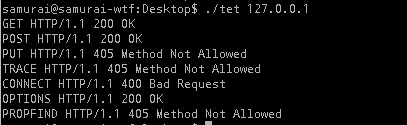
\includegraphics[width=\linewidth]{logos/methods.jpg}
	\caption{Results}
	\label{fig:test}
\end{figure}

\begin{figure}
	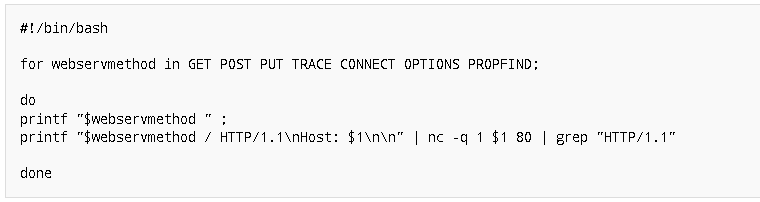
\includegraphics[width=\linewidth]{script.png}
	\caption{Script used for testing}
	\label{fig:script}
\end{figure}

\pagebreak
\subsection{Testing for SQL Injection (OTG-INPVAL-005) and Mysql testing (OTG-INPVAL-005)}\


\begin{tabular}{cR{12cm}}
	\textbf{Team2} & Likelihood: 0\\& Impact: 0\\& Risk: 0
\end{tabular}

\begin{tabular}{ l|p{11cm}  }
	\hline
	\multicolumn{2}{c}{\textbf{Team2}} \\
	\hline
	Observation   & We observed that no SQL Injection was possible. Since we knew that the other team had
	to use Mysql we tested also specifically for Mysql \\
	Discovery  & We tried inserting various SQL statements in the fields of using \textit{sqlmap} tool and failed, also we did static test of the PHP code using \textit{RIPS} which did not find any.\\
	Likelihood & N/A \\
	Implication    & N/A \\
	Recommendations & N/A \\
	Comparison& Our web application is also immune to SQL Injections \\
	\hline
\end{tabular}
\begin{figure}[ht!]
	\centering
	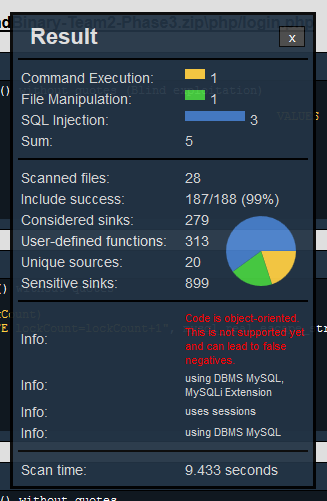
\includegraphics[width=50mm]{logos/RIPS2.jpg}
	\caption{RIPS \label{overflow}}
\end{figure}
Using \textit{RIPS} with verbosity level 1  and vulnerability all server-side we get the above results.
The 3 cases of \textit{SQL Injection} are \textit{false-positives}. The input in the query is already set and is not affected by the user input.
\begin{figure}[ht!]
	\centering
	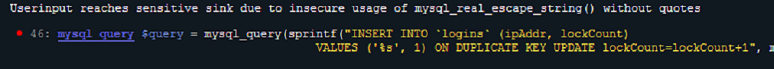
\includegraphics[width=150mm]{logos/Injection1.jpg}
	\caption{RIPS \label{overflow}}
\end{figure}

The case of file manipulation is \textit{false-positive} since the variables passed as parameters here have nothing to do with user input.
\begin{figure}[H]
	\centering
	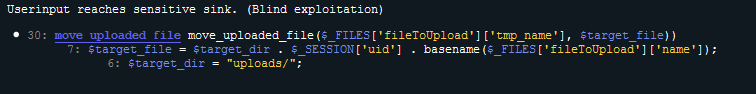
\includegraphics[width=150mm]{logos/file1.jpg}
	\caption{RIPS \label{overflow}}
\end{figure} 

Also using the following \textit{sqlmap} command we did not find any SQL Injection possible.\\

\begin{lstlisting}
sqlmap -u https://localhost/ex1/securecoding/
\end{lstlisting}
\begin{figure}[ht!]
	\centering
	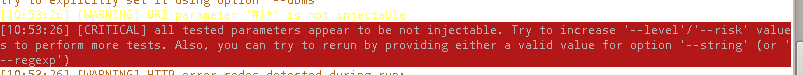
\includegraphics[width=150mm]{logos/sql.jpg}
	\caption{RIPS \label{overflow}}
\end{figure}
\pagebreak
\subsubsection{Team3}
Using \textit{RIPS} with verbosity level 1  and vulnerability all server-side we get the above results.
\begin{figure}[H]
	\centering
	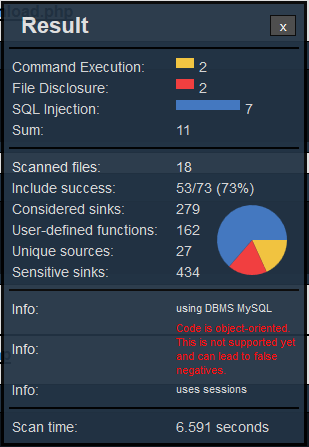
\includegraphics[width=50mm]{logos/stats3.jpg}
	\caption{RIPS \label{overflow}}
\end{figure}


For the \textit{SQL Injection} cases the input data is sanitized before being executed into the queries. So the warnings given by \textit{RIPS} are \textit{false-positive}.

Also using the following \textit{sqlmap} command we did not find any SQL Injection possible.\\

\begin{lstlisting}
sqlmap -u https://localhost/SecureCoding-Group3/online_banking/
\end{lstlisting}
\begin{figure}[ht!]
	\centering
	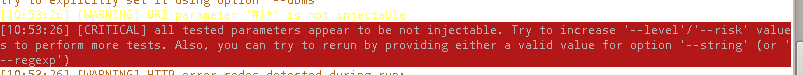
\includegraphics[width=150mm]{logos/sql.jpg}
	\caption{RIPS \label{overflow}}
\end{figure}



 
\pagebreak
\subsection{Testing for Code Injection, Testing for Local File Inclusion, Testing for Remote File Inclusion(OTG-INPVAL-012)}\

\begin{tabular}{cR{12cm}}
	\textbf{Team2} & Likelihood: 0\\& Impact: 0\\& Risk: 0
\end{tabular}

\begin{tabular}{ l|p{11cm}  }
	\hline
	\multicolumn{2}{c}{\textbf{Team2}} \\
	\hline
	Observation   & We did not find any vulnerability regarding code injection and local or remote file inclusion.  \\
	Discovery  & Tried to perform a command execution via the backticks (`) and also the semicolon (;) in the filename but our	webapp correctly handled the files without injections. We upload files with code written in them but nothing happened. \\
	Likelihood & N/A \\
	Implication    & N/A \\
	Recommendations & N/A \\ 
	\hline
\end{tabular}
\\
\vspace{0.5cm}
\\
\begin{tabular}{cR{12cm}}
	\textbf{Team3} & Likelihood: 0\\& Impact: 0\\& Risk: 0
\end{tabular}

\begin{tabular}{ l|p{11cm}  }
	\hline
	\multicolumn{2}{c}{\textbf{Team3}} \\
	\hline
	Observation   & We did not find any vulnerability regarding code injection and local or remote file inclusion in our web app.   \\
	Discovery  & Tried to perform a command execution via the backticks (`) and also the semicolon (;) in the filename but our	webapp correctly handled the files without injections. We upload files with code written in them but nothing happened. \\
	Likelihood & N/A \\
	Implication    & N/A \\
	Recommendations & N/A \\ 
	\hline
\end{tabular}
\pagebreak
\subsection{Testing for Command Injection(OTG-INPVAL-013)}\
\subsubsection{Team2}
The case of command execution is yet again a \textit{false-positive} since the variable entered into the \textit{exec} function is a file. If the file contains malicious user input is another problem, and we have to do the check for that elsewhere.\\

\begin{figure}[H]
	\centering
	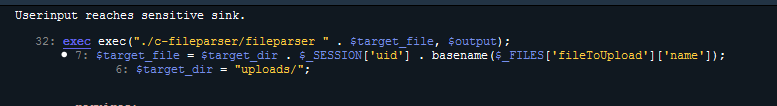
\includegraphics[width=150mm]{logos/command1.jpg}
	\caption{RIPS \label{overflow}}
\end{figure}
 
\pagebreak
\subsubsection{Team3}
\textit{RIPS} finds two vulnerabilities for file disclosure and command execution in \textit{applicationDownload.php}, which are \textit{false-positive} since the variable is taken from the database, the user does not input it directly.
\begin{figure}[H]
	\centering
	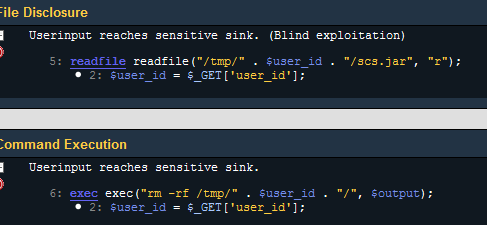
\includegraphics[width=50mm]{logos/download3.jpg}
	\caption{RIPS \label{overflow}}
\end{figure}
\textit{RIPS} finds two vulnerabilities for file disclosure and command execution in \textit{customer.inc.php}, the same case applies here, they are \textit{false-positive} the variables passed on the sensitive functions are not user input.
\begin{figure}[H]
	\centering
	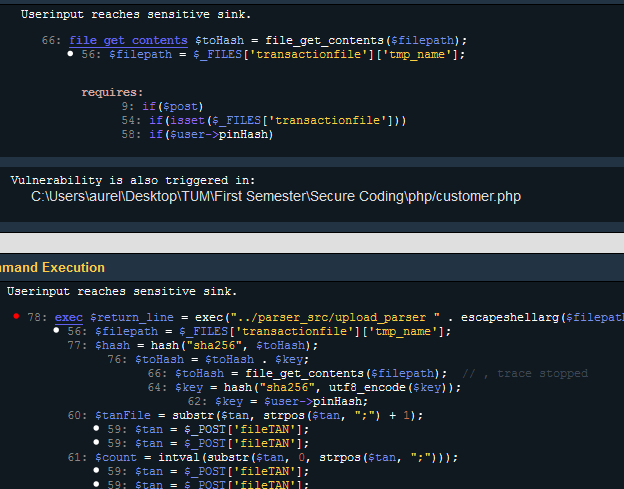
\includegraphics[width=150mm]{logos/trans3.jpg}
	\caption{RIPS \label{overflow}}
\end{figure}
\pagebreak
\subsection{Testing for Buffer overflow, Testing for Heap overflow, Testing for Stack overflow, Testing for Format string (OTG-INPVAL-014)}\

\begin{tabular}{cR{12cm}}
	\textbf{Team2} & Likelihood: 0\\& Impact: 0\\& Risk: 0
\end{tabular}

\begin{tabular}{ l|p{11cm}  }
	\hline
	\multicolumn{2}{c}{\textbf{Team2}} \\
	\hline
	Observation   & We did not find any vulnerability regarding buffer overflow,
	heap overflow, stack overflow or string formatting\\
	Discovery  & We used w3af to locate such vulnerabilities. \\
	Likelihood & N/A \\
	Implication    & N/A \\
	Recommendations & N/A \\ 
	\hline
\end{tabular}
\\
\vspace{0.5cm}
\\
\begin{tabular}{cR{12cm}}
	\textbf{Team3} & Likelihood: 0\\& Impact: 0\\& Risk: 0
\end{tabular}

\begin{tabular}{ l|p{11cm}  }
	\hline
	\multicolumn{2}{c}{\textbf{Team3}} \\
	\hline
	Observation   & We did not find any vulnerability regarding buffer overflow,
	heap overflow, stack overflow or string formatting\\
	Discovery  & We used w3af to locate such vulnerabilities. \\
	Likelihood & N/A \\
	Implication    & N/A \\
	Recommendations & N/A \\ 
	\hline
\end{tabular}
\pagebreak
\subsection{Testing for incubated vulnerabilities(OTG-INPVAL-015)}\

\begin{tabular}{cR{12cm}}
	\textbf{Team2} & Likelihood: 0\\& Impact: 0\\& Risk: 0
\end{tabular}

\begin{tabular}{ l|p{11cm}  }
	\hline
	\multicolumn{2}{c}{\textbf{Team2}} \\
	\hline
	Observation   &The webapp is secure towards incubated vulnerabilities.\\
	Discovery  & We tried XSS, uploading file with commands, SQL Injections and neither of them worked. So there is no possibility to inject code.\\
	Likelihood & N/A \\
	Implication    & N/A\\
	Recommendations & N/A \\ 
	\hline
\end{tabular}
\\
\vspace{0.5cm}
\\
\begin{tabular}{cR{12cm}}
	\textbf{Team3} & Likelihood: 0\\& Impact: 0\\& Risk: 0
\end{tabular}

\begin{tabular}{ l|p{11cm}  }
	\hline
	\multicolumn{2}{c}{\textbf{Team3}} \\
	\hline
	Observation   & We did not find any vulnerability regarding incubated vulnerabilities.\\
	Discovery  & There is no possibility to inject code in the webapp since every user input is sanitized \\
	Likelihood & N/A \\
	Implication    & N/A \\
	Recommendations & N/A \\ 
	\hline
\end{tabular}
\pagebreak
\section{Error Handling}\

\textbf{Team2}\\

Team2 provides an error for the transactions using file upload only when the file format is not correct. Every other time when the correct file format is uploaded with incorrect data, the file is accepted even though no transaction is executed.\\
 
 \pagebreak
\section{Business Logic Testing}\
\subsection{Test Business Logic Data Validation(OTG-BUSLOGIC-001)}\

\begin{tabular}{cc}
	\textbf{Team2} \hspace{9cm} & \begin{tabular}{@{}c@{}c@{}}Likelihood: 0\\ Impact: 0\\ Risk:0 \end{tabular}
\end{tabular}\

\begin{tabular}{ l|p{11cm}  }
	\hline
	\multicolumn{2}{c}{\textbf{Team2}} \\
	\hline
	Observation   & Tests show that data validation is both: client side and server side.\\
	Discovery  & We intercepted the input before it gets send to the server using \textit{Burp} and manipulated the data, and we received an error message. \\

	Likelihood & N/A \\
	Implication    & N/A \\
	Recommendations & N/A \\ 
	\hline
\end{tabular}
\\
\vspace{0.5cm}
\\
\begin{tabular}{cR{12cm}}
	\textbf{Team3} & Likelihood: 0\\& Impact: 0\\& Risk: 0
\end{tabular}

\begin{tabular}{ l|p{11cm}  }
	\hline
	\multicolumn{2}{c}{\textbf{Team3}} \\
	\hline
		Observation   & Tests show that data validation is both: client side and server side.\\
		Discovery  & We intercepted the input before it gets send to the server using \textit{Burp} and manipulated the data, and we received an error message. \\ 
		Likelihood & N/A \\
		Implication    & N/A \\
		Recommendations & N/A \\ 
	\hline
\end{tabular}
\pagebreak
 
\subsection{Test Number of Times a Function Can be Used Limits(OTG-BUSLOGIC-005)}\

\begin{tabular}{cc}
	\textbf{Team2} \hspace{9cm} & \begin{tabular}{@{}c@{}c@{}}Likelihood: 0\\ Impact: 0\\ Risk:0 \end{tabular}
\end{tabular}\

\begin{tabular}{ l|p{11cm}  }
	\hline
	\multicolumn{2}{c}{\textbf{Team2}} \\
	\hline
	Observation   & We tried inserting the same tan multiple times.\\
	Discovery  & The web application did not accept requests with a TAN that was already used in the HTML form, but we did not receive any error with the file upload, but the transaction did not go through. \\ 
	Likelihood & N/A \\
	Implication    & N/A \\
	Recommendations & N/A \\ 
	\hline
\end{tabular}
\\
\vspace{0.5cm}
\\
\begin{tabular}{cR{12cm}}
	\textbf{Team3} & Likelihood: 0\\& Impact: 0\\& Risk: 0
\end{tabular}

\begin{tabular}{ l|p{11cm}  }
	\hline
	\multicolumn{2}{c}{\textbf{Team3}} \\
	\hline
	Observation   & Tests show that data validation is both: client side and server side.\\
	Discovery  & We intercepted the input before it gets send to the server using \textit{Burp} and manipulated the data, and we received an error message. \\ 
	Likelihood & N/A \\
	Implication    & N/A \\
	Recommendations & N/A \\ 
	\hline
\end{tabular}

\pagebreak
\subsection{Test Upload of Unexpected File Types (OTG-BUSLOGIC-008) }
\begin{tabular}{cR{12cm}}
	\textbf{Team2} & Likelihood: 0\\& Impact: 0\\& Risk: 0
\end{tabular}

\begin{tabular}{ l|p{11cm}  }
	\hline
	\multicolumn{2}{c}{\textbf{Team2}} \\
	\hline
	Observation   & The is no possibility to upload any unexpected file type.  \\
	Discovery  & We tried to upload different type of files from the one presented on the website. There was an error every time the file had different extension from the one specified on the website.  \\
	Likelihood &  N/A \\
	Implication    & N/A \\
	Recommendation & N/A \\
	\hline
\end{tabular}
\\
\vspace{0.5cm}
\\
\begin{tabular}{cR{12cm}}
	\textbf{Team3} & Likelihood: 0\\& Impact: 0\\& Risk: 0
\end{tabular}

\begin{tabular}{ l|p{11cm}  }
	\hline
	\multicolumn{2}{c}{\textbf{Team3}} \\
	\hline
	Observation   & The is no possibility to upload any unexpected file type.  \\
	Discovery  & We tried to upload different type of files from the one presented on the website. There was an error every time the file had different extension from the one specified on the website.  \\
	Likelihood &  N/A \\
	Implication    & N/A \\
	Recommendation & N/A \\
	\hline
\end{tabular}
\pagebreak
 
\section{Client Side Testing}
\subsection{Testing for Clickjacking (OTG-CLIENT-009) }
\begin{tabular}{cR{12cm}}
	\textbf{Team2} & Likelihood: 8\\& Impact: 9\\& Risk: 8
\end{tabular}

\begin{tabular}{ l|p{11cm}  }
	\hline
	\multicolumn{2}{c}{\textbf{Team2}} \\
	\hline
	Observation   & We found a vulnerability in the web application that allows
	attackers to make clickjacking attacks by bundling the website
	inside an iframe to give the user the feeling of interacting with
	the target website but being instead on a malicious web page.  \\
	Discovery  & The tool w3af found out that the web application does not make
	use of protection techniques to prevent click jacking attacks.  \\
	Likelihood &  It is quite likely that someone would use this kind of exploits
	on an online banking website, because the people trust these
	websites. It is not very difficult to use this vulnerability to attack
	the users. \\
	Implication    & The user would think he would interact with the secure online
	banking system, but in reality he is on a malicious website that
	can record his interaction and filter out sensitive information. \\
	Recommendation & The use of X-Frame-Options header would help on the server side to
	prevent against this type of attacks, but is never used by this web
	application.  \\
	\hline
\end{tabular}
\\
\vspace{0.5cm}
\\
\begin{center}
	\begin{tabular}{ll}
		\rowcolor[HTML]{34CDF9}
		{\color[HTML]{ECF4FF} \textbf{Metric}}        & {\color[HTML]{ECF4FF} \textbf{Value : }} \\
		\rowcolor[HTML]{BBDAFF}
		{\color[HTML]{333333} Access Vector}          & {\color[HTML]{333333} } N              \\
		\rowcolor[HTML]{ECF4FF}
		{\color[HTML]{333333} Attack Complexity}      & {\color[HTML]{333333} } L              \\
		\rowcolor[HTML]{BBDAFF}
		{\color[HTML]{333333} Privileges Required}    & {\color[HTML]{333333} } N              \\
		\rowcolor[HTML]{ECF4FF}
		{\color[HTML]{333333} User Interaction}       & {\color[HTML]{333333} } R              \\
		\rowcolor[HTML]{BBDAFF}
		{\color[HTML]{333333} Scope}                  & {\color[HTML]{333333} } U              \\
		\rowcolor[HTML]{ECF4FF}
		{\color[HTML]{333333} Confidentiality Impact} & {\color[HTML]{333333} } H              \\
		\rowcolor[HTML]{BBDAFF}
		{\color[HTML]{333333} Integrity Impact}       & {\color[HTML]{333333} } H              \\
		\rowcolor[HTML]{ECF4FF}
		{\color[HTML]{333333} Availability Impact}    & {\color[HTML]{333333} } N
	\end{tabular}
\end{center} 
\vspace{0.5cm}

\begin{tabular}{cR{12cm}}
	\textbf{Team3} & Likelihood: 0\\& Impact: 0\\& Risk: 0
\end{tabular}

\begin{tabular}{ l|p{11cm}  }
	\hline
	\multicolumn{2}{c}{\textbf{Team3}} \\
	\hline
	Observation   & There is no possibility for clickjacking.  \\
	Discovery  &The use of X-Frame-Options header prevents this. \\
	Likelihood &  N/A \\
	Implication    & N/A \\
	Recommendation & N/A \\
	\hline
\end{tabular}

\appendix{}

 % TODO: remove if glossary not needed
\glsaddall{} % add all defined terms to glossary, even if not referenced in text
\printglossaries{}

\microtypesetup{protrusion=false}
%\listoffigures{}
%\listoftables{}
\microtypesetup{protrusion=true}
\printbibliography{}

\end{document}
